\chapter{Automatic extraction the morphometry landmarks by Convolutional Neural Network}
In the content of this chapter, we studied on the articles: \textbf{Deep Convolutional Network Cascade for Facial Point Detection}\cite{sun2013deep} (Yi Sun et al) and \textbf{Automatic ear detection and feature extraction using Geometric Morphometrics and Convolutional neural networks}\cite{cintas2016automatic} (Celia Cintas et al). Both of articles proposed the specific to automatic identification the landmarks on human face and human ears. Besides the studying, we also tried to apply the networks to estimated the landmark on the pronotum dataset \cite{}.
\section{Facial Point Detection by CNN}
Yi Sun et al proposed a method to estimate the position of five facial keypoints: left eye center, right eye center, nose tip, left mouth corner and right mouth corner (called landmarks). The proposed method includes 3-levels designed convolutional networks.
\subsection{Data}
The dataset with 13466 face images includes 5590 images from LFW \cite{huang2007labeled} and remaining images are downloaded from the web. The dataset is divided into training set with 10000 images and validation set with 33466 images. Each face is labeled with five landmarks and bounding box is created around the face. It was used as the input at the F1 network of the first level. At other networks, the bounding boxes are also used to limit the training region but with different size.
\subsection{Model}
\begin{figure}[h]
	\centering
	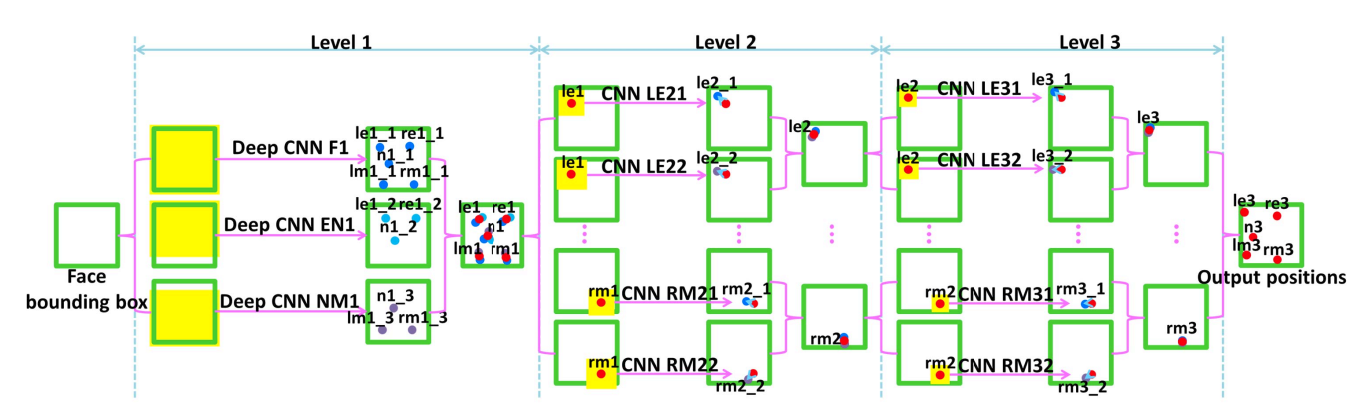
\includegraphics[scale=0.3]{images/3levels}
	\caption{The 3-levels proposed architecture}
	\label{3levels}
\end{figure}
They cascade three levels of convolutional networks to make the prediction (Fig. \ref{3levels}). The first level in architecture is designed to detect multiple landmarks, two last levels are designed to verify the position of each landmark.

At the first level, three CNNs are employed to study the location of the facial points: F1, EN1, NM1 whose input regions cover the whole face (F1), eyes and nose (EN1), nose and mouth (NM1). Each network predicts the landmarks corresponding with the region that it covers. At the end of level 1, the coordinate of each landmark is average of coordinates that predicted from three networks.
\begin{figure}[h]
	\centering
	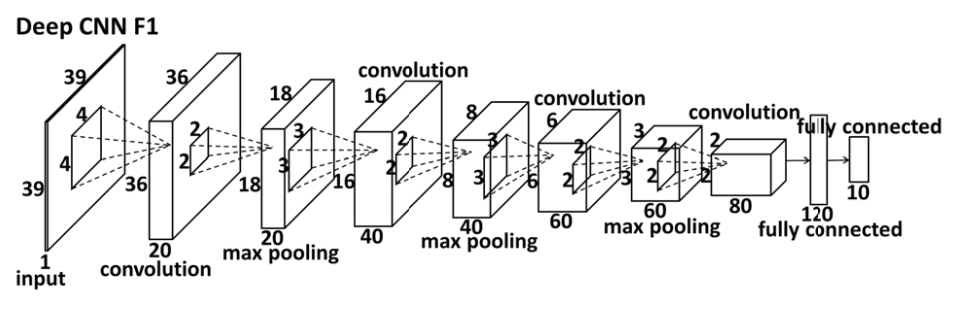
\includegraphics[scale=0.3]{images/1Fconv}
	\caption{The structure of F1-convolutional network}
	\label{1Fconv}
\end{figure}
Fig. \ref{1Fconv} illustrates the deep structure architecture of F1 network, which contains four convolutional layers followed by max pooling and two full connected layers. The structure architecture of EN1 and NM1 are also the same with the structure of F1. The only difference is the different size at each layer because the size of the input regions are different.

The networks at the second and third levels take local patches centered at the predicted position of previous levels as input and are allowed to make small changes to previous prediction. The size of patches are also reduced along with the cascade model. For each position, two networks are used to predict the new positions and the last predicted position is average of the new positions. With 3-levels model, the purpose of the networks at the first level are estimated the landmark positions with large errors; the networks at last two levels are designed to achieve high accuracy.
\subsection{Experiments}
\subsubsection{Training}
At the first level, the patches according the bounding boxes are used as the input of the networks. At the following levels, the patches centered at previous predicted position is used to train. The size of the patches is decreased for each level. The learnable parameters include weight w, the gain g and the bias b which are initialized by small random number and learned by stochastic gradient descent.

The detection error on each facial point is measured by Eq. \ref{eq1}. If the error is greater than $5\%$, it is considered as failure.
\begin{equation}
	err = \sqrt{(x-x')^2 + (y-y')^2}/l
	\label{eq1}
\end{equation}
Where:
\begin{itemize}
	\item l is the width of the bounding box around the face.
	\item $(x,y)$ is ground truth facial point
	\item $(x',y')$ is predicted position
\end{itemize}
\subsubsection{Testing}
The model is tested with a dataset of 2557 face images. The image with the bounding box of the face is used as the input of the model. At the end, the predicted position is estimated from the model. By using the way in Eq.(\ref{eq1}) to evaluate the model, the error statistic on each level is obtained.
\begin{figure}[h]
	\centering
	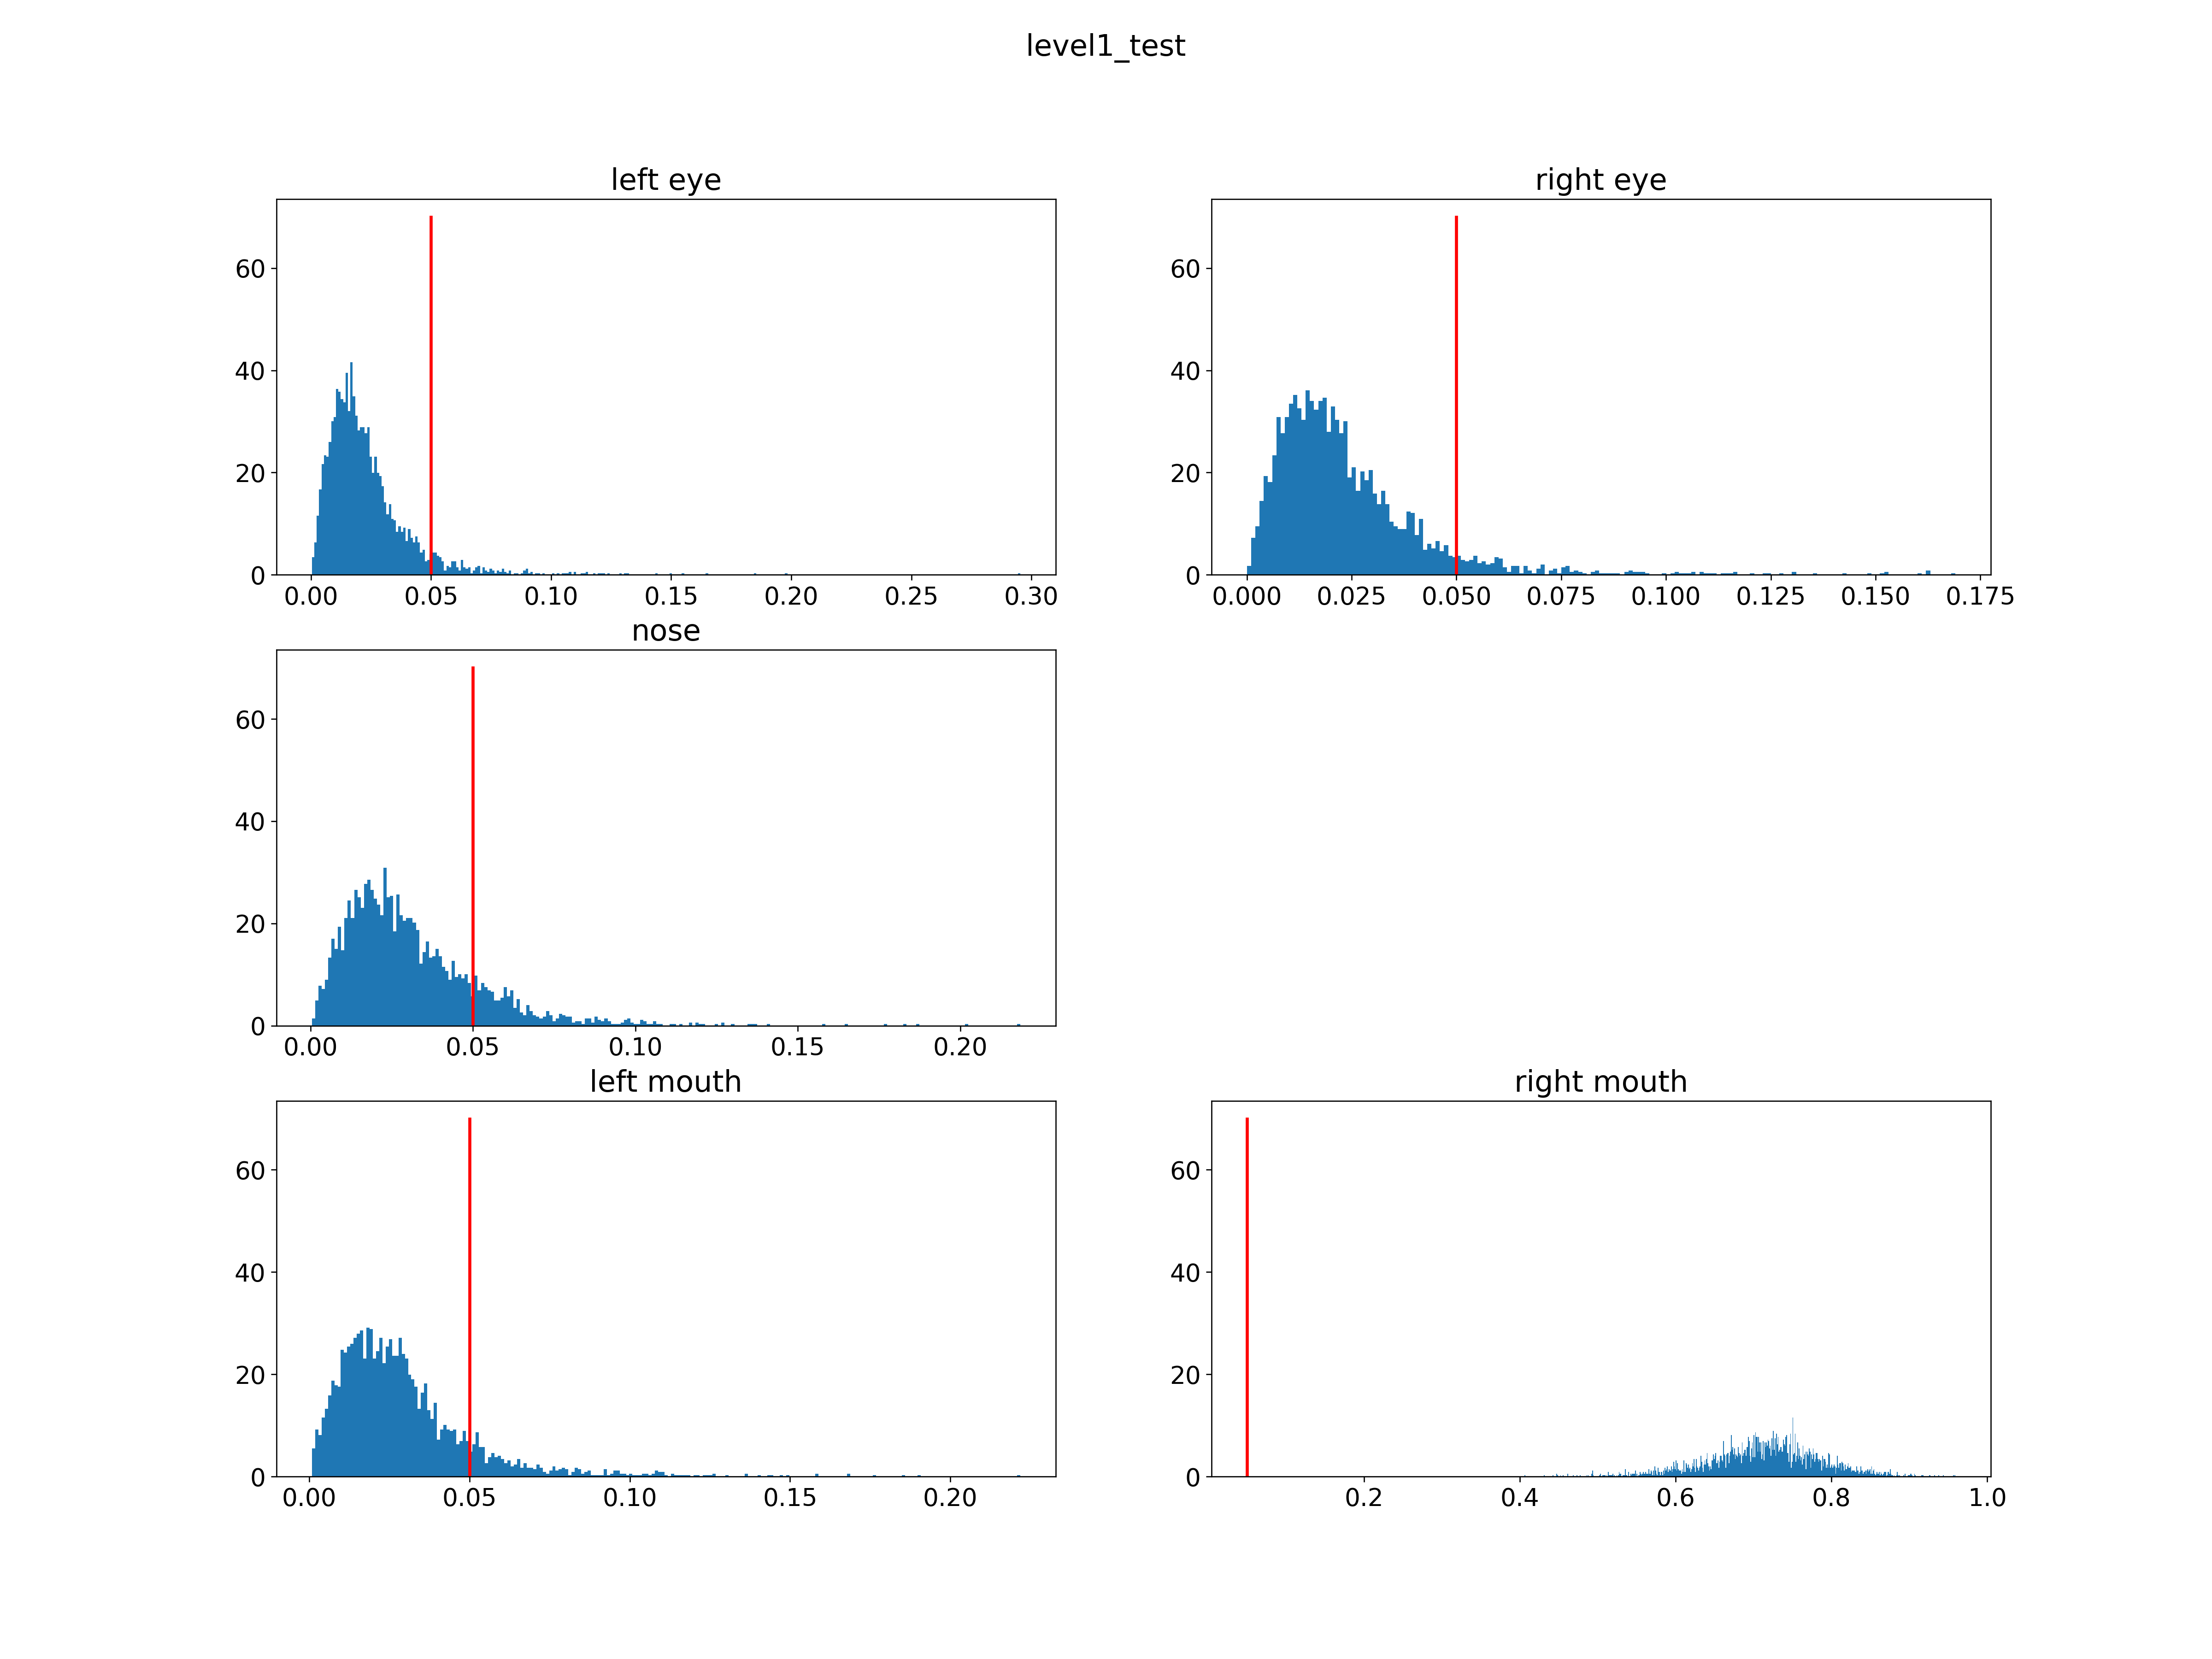
\includegraphics[scale=0.3]{images/level1_test}
	\caption{The error on each landmark in level 1}
	\label{1Fconv}
\end{figure}
\begin{figure}[h]
	\centering
	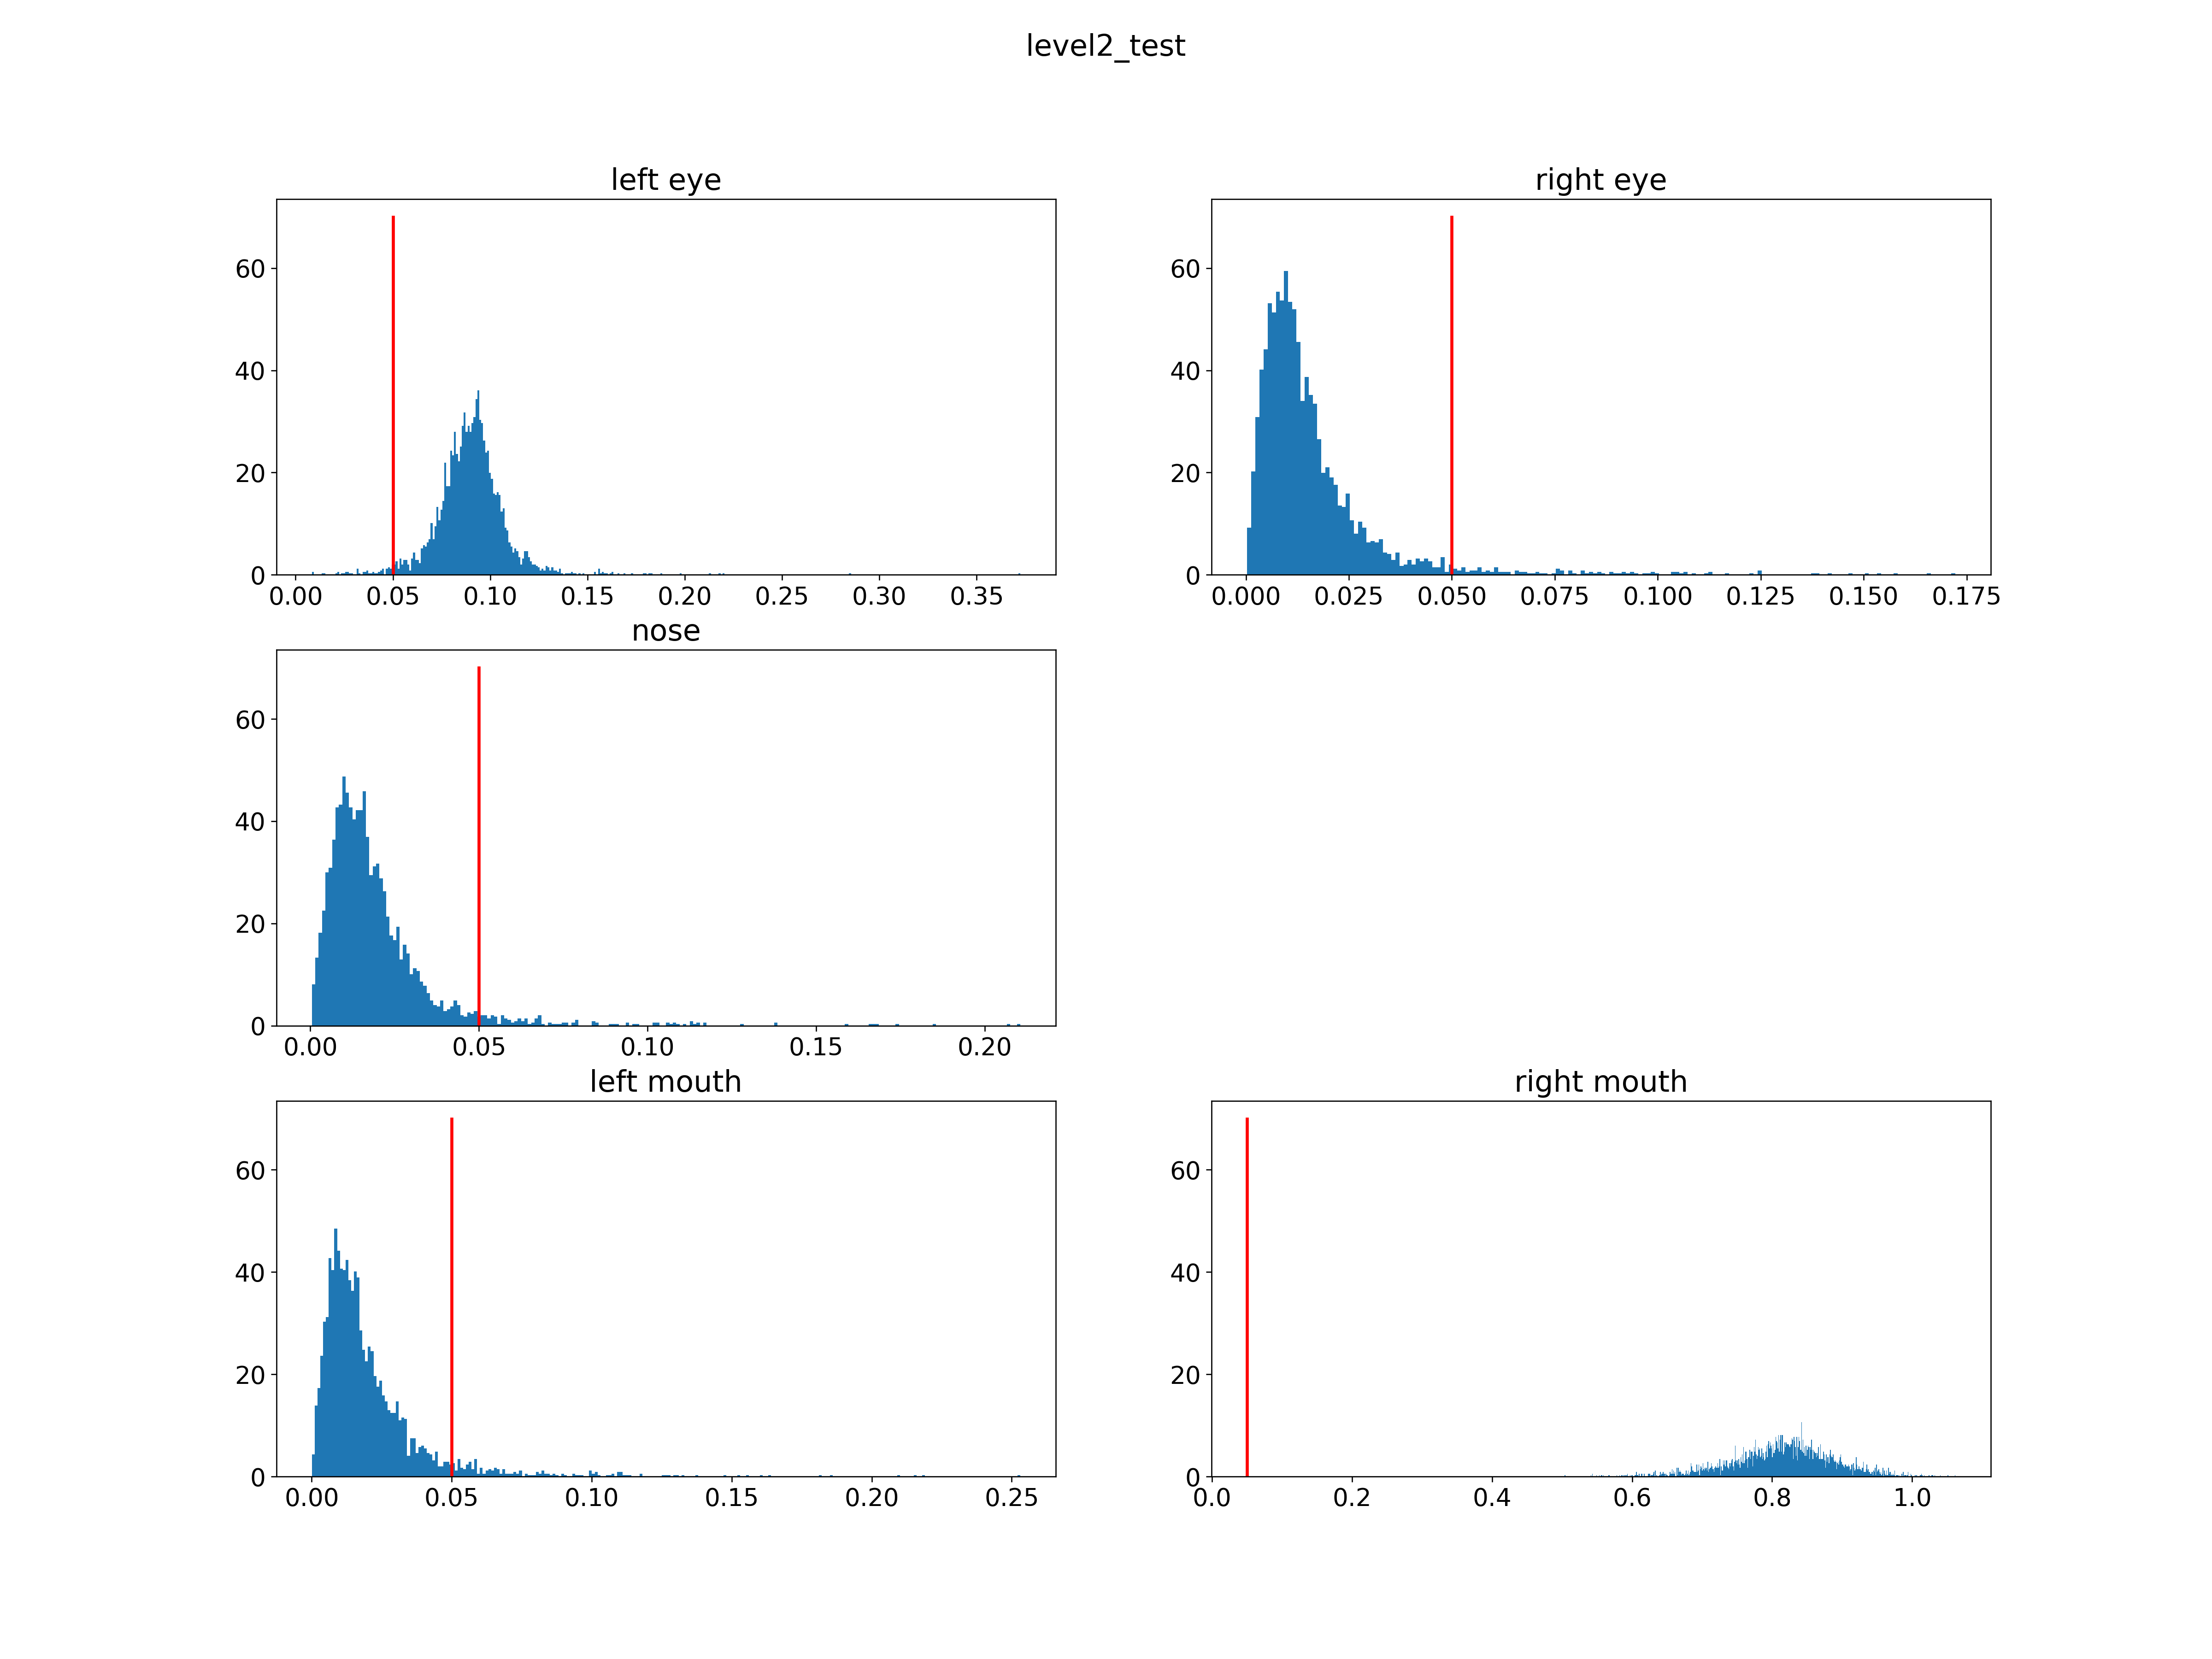
\includegraphics[scale=0.3]{images/level2_test}
	\caption{The error on each landmark in level 2}
	\label{1Fconv}
\end{figure}
\begin{figure}[h]
	\centering
	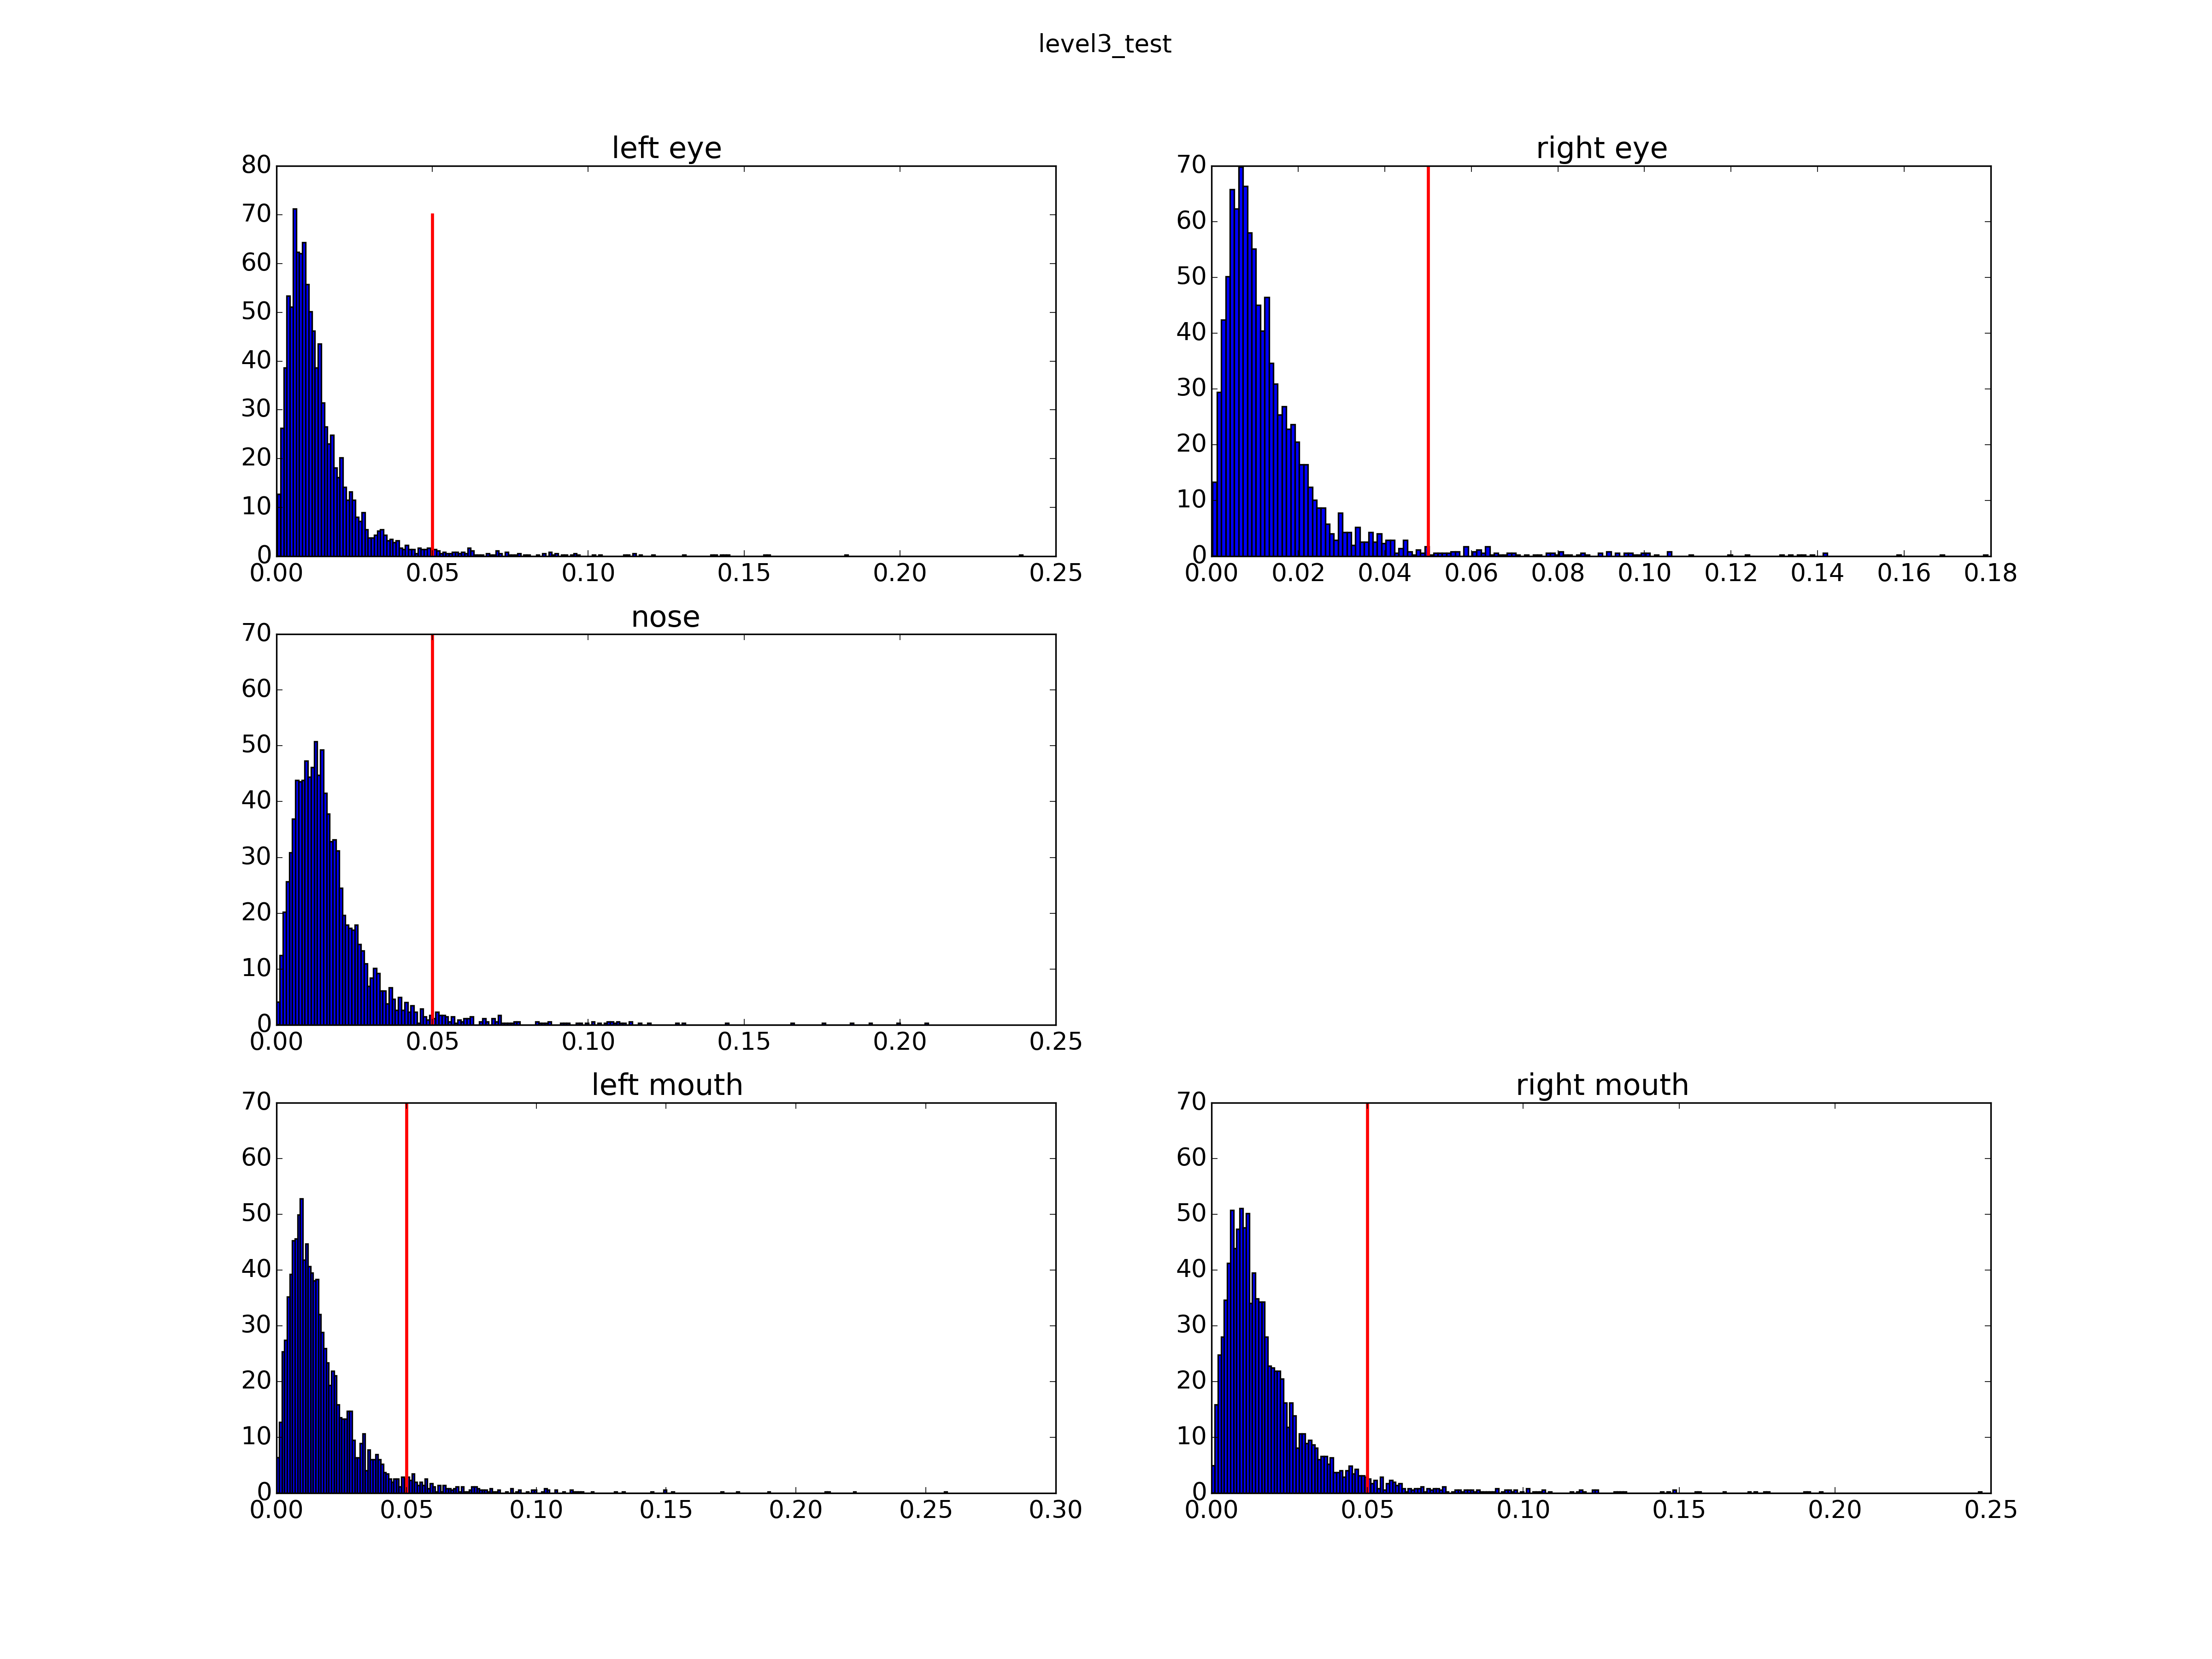
\includegraphics[scale=0.3]{images/level3_test}
	\caption{The error on each landmark in level 3}
	\label{1Fconv}
\end{figure}
According the charts, all the facial points are detected with high accuracy at all levels (except right mouth in level 1,2).
\subsection{Model with pronotum landmarks data}
The networks in the first level is modified to suitable with the prediction of landmarks on pronotum. For each pronotum, eight manual landmarks have been set. The bounding box is created depending on the coordinate of the manual landmark. The networks in the first level are used as followed:
\begin{itemize}
	\item F1 network recognizes whole pronotum bounding box with eight landmarks.
	\item EN1 network predicts the location of the first five-landmarks.
	\item NM1 network is used to estimated the position of last four-landmarks.
	\item At the end, the position of each landmark is average of the predicted position in the networks.
\end{itemize} 
\subsubsection{Data and training}
The dataset includes 293 pronotum images. The images are divided into three subset: training set (200 images), validation set (60 images) and test set (33 images). To enlarge the dataset during training, the image in training and validation set are augmentation by modifying the valued of red and green channel. So, at the end, we have 600 and 180 images in training and validation set, respectively.
\subsubsection{Testing}
The error rate of each network during training is shown in the table:\\
\begin{table}[h!]
	\centering
	\begin{tabular}{l r}
	Network & Loss \\ \hline
	F1 & 0.013 \\ \hline
	EN1 & 0.47\\ \hline
	NM1 &  0.5
	\end{tabular}
\end{table}\\
The model is tested on four images. The position of the landmark is located.
\begin{figure}[h!]
\centering
\subfloat[Test 1]{\label{}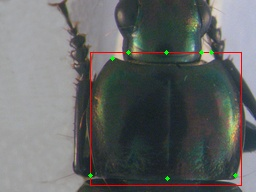
\includegraphics[width=0.45\textwidth]{./images/test1}}~~
\subfloat[Test 2]{\label{}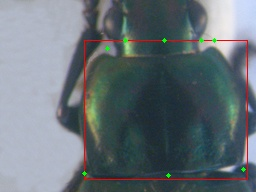
\includegraphics[width=0.45\textwidth]{./images/test2}}\\
\subfloat[Test 3]{\label{}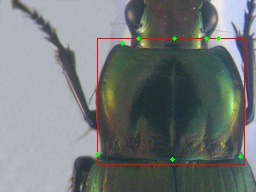
\includegraphics[width=0.45\textwidth]{./images/test3}}~~
\subfloat[Test 4]{\label{}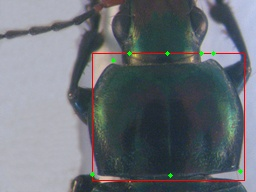
\includegraphics[width=0.45\textwidth]{./images/test4}}\\
\caption{The pronotum with predicted landmarks at level 1}
\label{figcentroidSize}
\end{figure}

Next: continue with the network of level 2, 3.
\section{Automatic ear detection with CNN}
Celia Cintas et al \cite{•} proposed a method based on Geometric Morphometric and Deep Learning for automatic ear detection and feature extraction in the form of landmarks. The convolutional neural network was trained with a set of manually landmarks examples. The network is able to provide the morphometric landmarks on ear image automatically.
\subsection{Dataset}
The image and manual landmark belong to the CANDELA initiative \cite{•}, a project includes geneticists, bioinformatics and social-anthropologists interested on Latin American. CANDELA contains 7500 images with the size of $2136 \times 3216$. The provided dataset contains 2753 images which extracted from the CANDELA dataset. For each image, a set of 45 landmarks and semi-landmarks provided by human operators. The dataset was split into a training set with 2051 images (75\%) and a validation set of 684 images (25\%).
\subsection{Network}
Three models were designed and trained for performing the automatic landmarks task.  These architectures are different in the number of convolution layers, the filter sizes, and the learning rate. An image with a single channel of the size  $96 \times 96$ with brightness scaled to [0,1], is taken as the input of the network. Fig.\ref{1Econv} shows the best architecture. In this architecture, a structure of two convolutional layers with the filters, followed by maximum pooling and dropout layer. This structure is repeated three times to obtain features at different levels with different size of filters. After extraction the features, two fully connected linear layers with 1500 units each and a dropout layer is hired. The output layer contains 90 output units (corresponding with 45 landmarks) for the predicted position of the landmarks. The implementation used Python and the Lasagne library \cite{}
\begin{figure}[h!]
	\centering
	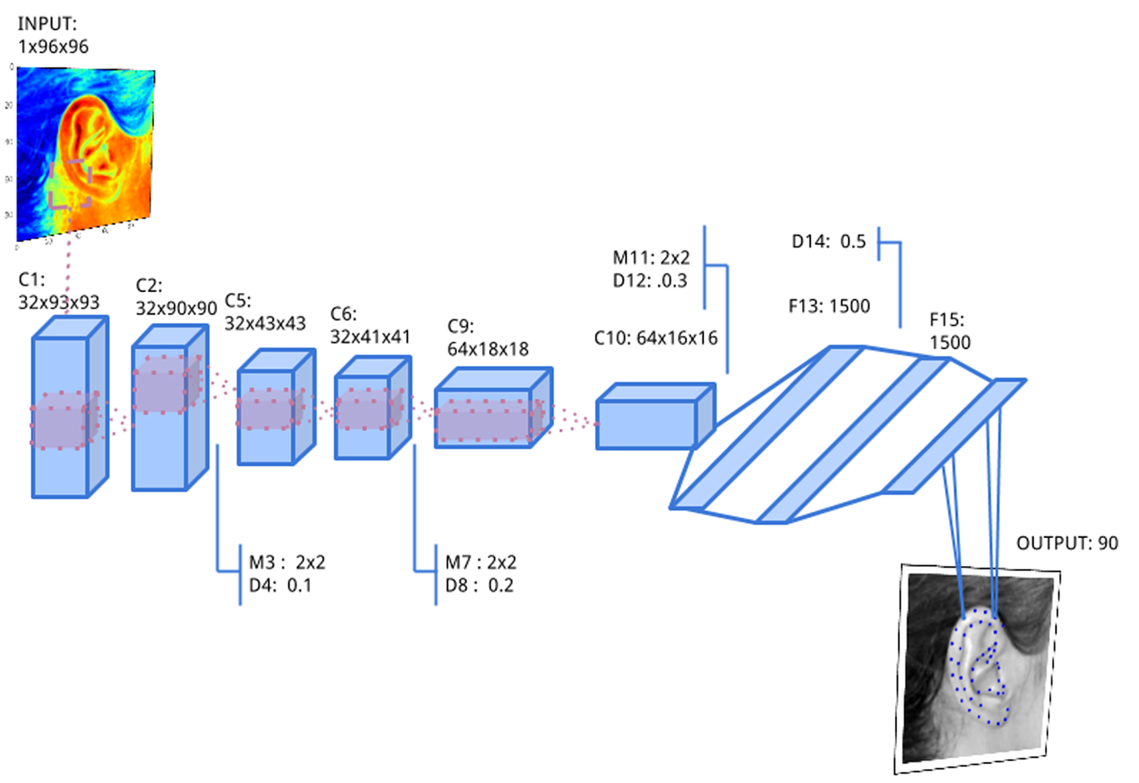
\includegraphics[scale=0.27]{images/ear_cnn}
	\caption{The best architecture for automatic ear's landmarks detection}
	\label{1Econv}
\end{figure}
\subsection{Experiments}
Following the article, the method is evaluated the usual quality metrics for regression problems, in particular $r^2$, root mean square error (RMSE), explained variance (EV), and Pearson's correlation. The accuracy of three architectures are shown in Table \ref{tbear1}. Also, in Table \ref{tbear2}, the RMSE for each landmarks is shown. The regression metrics were computed using \textit{scikit-learn}\cite{}.
\begin{table}[h!]
	\centering
	\begin{tabular}{l c c c}
	& Arch0 & Arch1 & Arch2 \\ \hline
	$r^2$ & 0.709 & 0.678 & 0.698 \\ \hline
	RMSE & 2.296 & 2.415 & 2.338\\ \hline
	EV & 0.976 & 0.974 &  0.975 \\ \hline
	Pearson & 0.988 & 0.987 &  0.988 \\ \hline	
	\end{tabular}
	\caption{Performance of three different ConvNet architectures}
	\label{tbear1}
\end{table}\\
\begin{table}[h!]
	\centering
	\begin{tabular}{l r}
	\# Landmark & RMSE \\ \hline
	1 & 1.8183 \\ \hline
	2 & 1.2216\\ \hline
	3 &  1.08651\\ \hline
	4 &  1.3291\\ \hline
	5 &  2.4477\\ \hline
	6 &  2.59746\\ \hline
	7 &  1.17571\\ \hline
	\end{tabular}
	\caption{RMS error for each landmark}
	\label{tbear2}
\end{table}\\
Because the CANDELA dataset is not open. Another dataset was chosen to study the network. The new dataset was used for the Facial Keypoint Detection including 7049 gray-scale images ($96 \times 96$). For each image, we are supported learn to find the position of 15 landmarks. After dropping some missing data, the dataset remains 2140 images. All the images with coordinates of manual landmarks is stored in csv file and fetched into the network. The training and validation loss are shown in Fig. \ref{}.
\begin{figure}[h!]
	\centering
	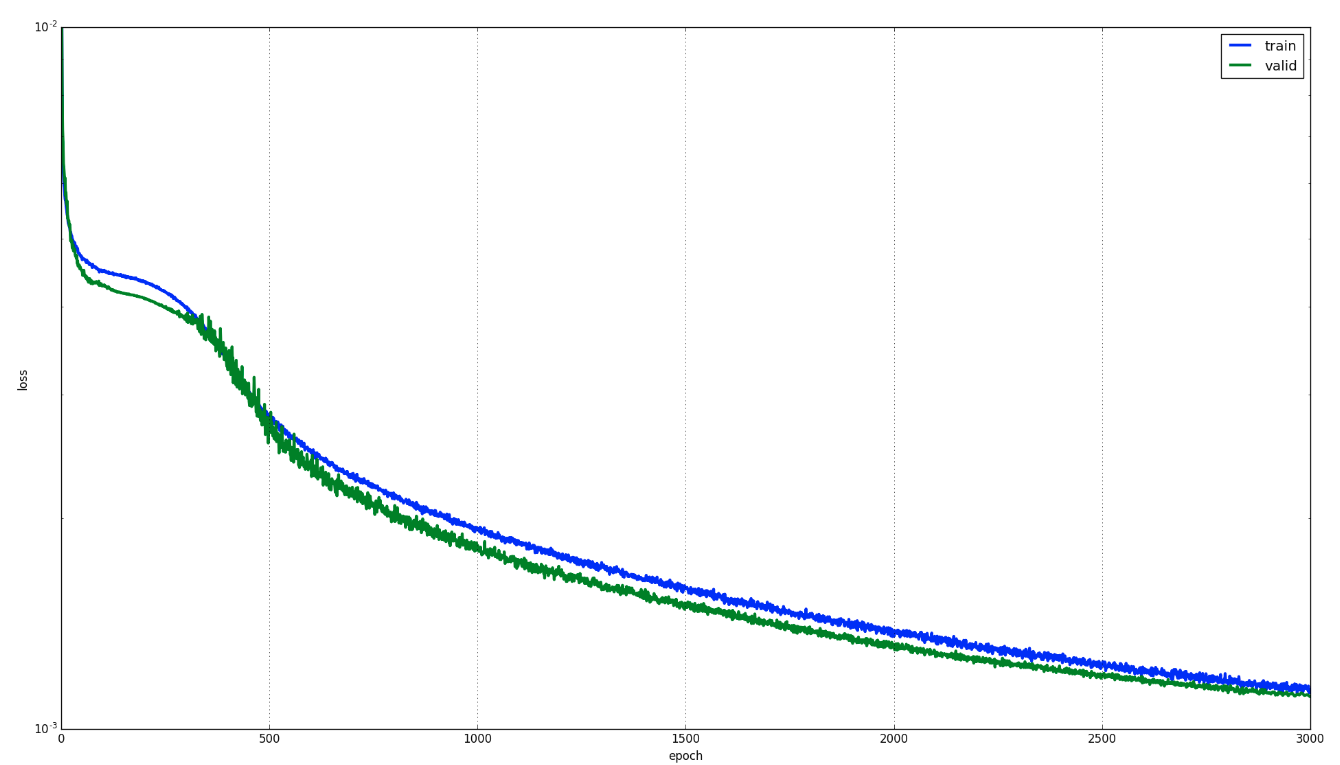
\includegraphics[scale=0.27]{images/trainloss}
	\caption{The loss of Ear-CNN network with facial point dataset}
	\label{1Econv}
\end{figure}